% The first part of a LaTex document is called the "header". In the header you specify rules for formatting and can define new commands. If you have some idea what you are doing, you should feel free to change this file. The worst that will happen is your document won't compile.


\documentclass[11pt]{amsart} % this command specifies the font-size and that we want to use the AMS (American Mathematical Society) article class.
\usepackage{amssymb, amsmath, amsthm} %this command loads in special ways of formatting theorems and additional mathematical symbols.
\usepackage{color} %this package allows you to use colored text
\usepackage{graphicx} %this package lets you include images

%-----------------------------------------------
% Here are some optional packages you may want to use at some point. To make use of them uncomment them.

%\usepackage[shortalphabetic]{amsrefs}  %this package allows a certain kind of bibliography style. You won't need it for typical homework assignments.
 

\usepackage{fourier} %this command changes the font. You can find the commands for other fonts online. Be sure to use one that includes the math symbols. This font was chosen so that the blackboard bold "1" will show up correctly.
\usepackage[T1]{fontenc}



\usepackage[hidelinks=true]{hyperref} % this command turns references and citations into links.
%\usepackage{pinlabel} %this is useful package for adding labels to figures.
%-----------------------------------------------


%-----------------------------------------------
%Define theorem styles

\theoremstyle{theorem} % this sets the overall style for the following environments
\newtheorem{theorem}{Theorem} %this is the environment for theorems. To enter the environment you type \begin{theorem} as in the example below. The second argument is the name that appears when the document is compiled.       
\newtheorem*{theorem*}{Theorem} %This produces an unnumbered theorem
\newtheorem{lemma}[theorem]{Lemma} %This is the lemma enviornment. The middle argument specifies that Lemmas and Theorems should be given the same numbering.
\newtheorem{definition}[theorem]{Definition}
%-----------------------------------------------

\newcommand{\spacing}{\parskip 6.6pt \parindent 0pt} %This specifies that paragraphs should not be indented and that there should be a space between paragraphs
\spacing


\newtheorem{innercustomthm}{Theorem}
\newenvironment{customthm}[1]
  {\renewcommand\theinnercustomthm{#1}\innercustomthm}
  {\endinnercustomthm}
\usepackage{float}
\usepackage{caption}
\begin{document} 


\textbf{Final Project:} Circuits in Graphs \\
\textbf{Date:} May 10, 2019 \\
\textbf{Author:} Iris Liu, Taryn Waite, and Curtis Zhuang

$\qquad$This project explores two applications of paths and circuits in graphs, the K\"{o}nisberg Bridge Problem and Hamiltonian paths in DNA reconstruction. All information was obtained from our course textbook \cite{Taylor}. 

\textbf{1. K\"{o}nisberg Bridge Problem and Eulerian circuits}

    $\qquad$An early application of what was to become graph theory was the \textbf{K\"{o}nisberg Bridge Problem} in 1732, when a question about paths and bridges was posed in the town of K\"{o}nisberg, Prussia. The town had seven bridges, and the question was whether it was possible to cross all of them without crossing any twice. 
    
    
    \begin{figure}[h]
    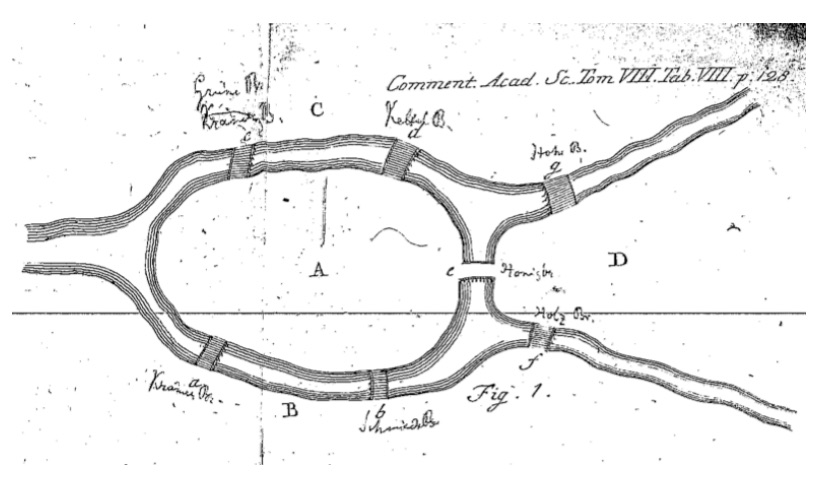
\includegraphics[width=60mm]{bridges.jpg} 
    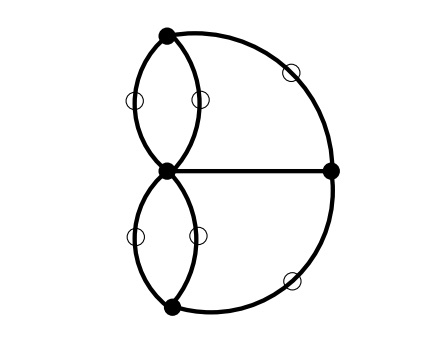
\includegraphics[width=50mm]{bridge_graph.jpg} 
    \caption*{Map of the K\"{o}nisberg bridges (left) and the corresponding graph \cite{Taylor}} 
    \end{figure}

	$\qquad$As shown above, the situation can be modeled with a graph, where each land mass is represented by a vertex and each bridge between land masses is represented by an edge. Since there are some land masses adjacent to more than once bridge, we add a vertex in the center of each bridge.

	$\qquad$Then, the problem is to determine whether there is an \textbf{Eulerian path} in the graph, which is a path that traverses each edge in the graph exactly once. Mathematician Leonhard Euler proved that, in the case of the K\"{o}nisberg Bridge Problem, no such path existed.

	$\qquad$The proof of the K\"{o}nigsberg Bridge Problem can done using contradiction. We suppose there exists a path that traverses each edge exactly once. In order for this to happen, for every vertex other than the starting and ending points, the path must enter and leave the vertex through two different edges, meaning that the vertices must be adjacent to an even number of edges. However, every vertex in the K\"{o}nigsberg Bridge graph is adjacent to an odd number of edges, so the path we are looking for must not exist.

	$\qquad$ From here, we can extend our question to the general conditions under which there exists an \textbf{Eulerian circuit}, which is an Eulerian path that is closed, in a graph. In order to answer this question, we will introduce the idea of \textbf{valence}, which is the number of edges that are not loops for which a vertex $v$ is an endpoint plus twice the number of loops adjacent to $v$. It turns out that graphs in which each vertex has an even valence contain Eulerian circuits. This is theorem 9.7.2, which we will prove later.


	\textbf{2. Hamiltonian Path and DNA Reconstruction}
	
	$\qquad$The idea of paths in graphs is also applied to current biologists' efforts to reconstruct DNA sequences. Long DNA strands are cut into fragments in order to be readable by technology; however, the cutting process does not preserve the order of the sequence, so in order to reconstruct the initial sequence, we need to cut multiple copies of it and compare the resulting fragments. For example, consider the DNA sequence 	
				\[
				TAATGCCA.
				\]
	Possible fragments that multiple copies of this sequence could be cut into include:
				\[
				TAA\enspace AAT\enspace ATG\enspace TGC\enspace GCC\enspace CCA.
				\]
				
	$\qquad$Looking at the fragments, TAA has two AA bases, which only appear again in the AAT fragment, we therefore know that 
				\[
				TAA\enspace AAT\enspace \Rightarrow TAAT.
				\]
	$\qquad$Following the exact same strategy, we are able to use all of the fragments to reconstruct the order of the original sequence:
				\[
				\begin{split}
				TAAT\enspace ATG\enspace &\Rightarrow TAATG \\
			     TAATG\enspace TGC\enspace &\Rightarrow TAATGC \\
			     TAATGC\enspace GCC\enspace &\Rightarrow TAATGCC \\
			     TAATGCC\enspace CCA\enspace &\Rightarrow TAATGCCA \\
				\end{split}
				\]
	$\qquad$Notice that we are able to reconstruct the sequence nicely because each time the overlapping bases only appear in one unvisited fragments; whereas, the presence of repeats could hinder the reconstruction process and lead to a wrong order. That is, at some point, we are not able to add unvisited fragments into the sequence and therefore to use every fragment, some kind of repetitions of fragments must be involved. 
	
	$\qquad$Observe that each fragment could be viewed as one vertex, and the overlapping bases, indicating possible adjacency of two fragments, could be viewed as directed edges, pointing from one fragment, or vertex, to another. The correct reconstruction should be a \textbf{Hamiltonian path}, which is a path where each vertex is visited only once, meaning that each fragment is only used once.  
	
	$\qquad$Notice that an Eulerian path crosses every edge exactly once, while a Hamiltonian path passes through each vertex exactly once. For a Hamiltonian path, there could be edges that are not visited, while an Eulerian path crosses every edge once but could pass through some vertices more than once.

\begin{customthm}{9.7.2}
    Suppose that G is a nonempty finite connected graph such that every vertex has even valence.
    Then G contains an Eulerian circuit.
\end{customthm}

    This theorem allows us to generalize the idea of the K\"{o}nisberg Bridge Problem to all graphs. We will first prove the theorem for graphs whose vertices all have valence 2. Note that this section of the proof is taken verbatim from \cite{Taylor}. Next, we will use this result to prove the theorem for graphs whose vertices all have even valence by using a proof by complete induction, where we induct on the number of vertices that have valence of at least 4. 

    \begin{proof}[Proof of Theorem 9.7.2]

    We begin by proving the theorem for graphs with the property that every
    vertex has valence 2. We prove this by minimal counter-example.


    Assume that G is a nonempty finite connected graph such that every vertex has valence 2. Assume,
    for a contradiction, that G does not contain an Eulerian circuit. Out of all such counter-examples, we
    may assume that we selected G to minimize the number of vertices. Since G is non-empty, it has a
    vertex v. By hypothesis, v is the endpoint of two (not necessarily distinct edges) $e_-$ and $e_+$. If $e_- = e_+$
    then, since G is connected, it is a loop. The path v, v is then an Eulerian circuit. If $e_- \neq e_+$, let $G'$ be the graph obtained from G by merging $e_-$ and $e_+$ into a single edge e and removing v as a vertex. Notice that since $e_-$ and $e_+$ had other endpoints, distinct from v as v had valence 2. Thus, $G'$ is still connected (do you see why?) and nonempty. It also has one less vertex than G. Thus, $G'$ cannot be a counterexample and so has an Eulerian circuit
    \[
    \alpha = v_0, v_1,..., v_n.
    \]
    Since $\alpha$ traverses every edge of $G'$ exactly once, there exists an $i \in \{0,...,n -1\}$ such that the ends of $\alpha$
    are the ends of e and these ends are $\{v_i , v_{i+1}\}$. Splitting e back into $e_-$ and $e_+$, the path
    \[
    v_0, v_1,..., v_i , v, v_{i+1},..., v_n.
    \]
    is then an Eulerian circuit in G. But this contradicts the fact that G is a counter-example to the theorem. Thus, the theorem holds for all nonempty finite connected graphs such that every vertex has valence 2.

    Now, we will prove that the theorem holds for nonempty finite connected graphs G with all vertices having even valence. We will use complete induction on the number of vertices with valence $\geq 4$.

    \underline{Base Case:} G has 0 vertices with valence $\geq 4$. In this case, since all vertices in G must have even valence and G must be connected, either G consists of one vertex with valence 0 or all of the vertices in G have valence 2. In the first case, there is an Eulerian path consisting of the vertex. In the second case, as proved above, G has an Eulerian circuit.

    \underline{Inductive Step:} Assume that for some $k \in \mathbb N \text{*}$, there exists an Eulerian circuit in all finite connected graphs that have $\leq k$ vertices with valence $\geq 4$. We will show that if G has $k+1$ vertices with valence $\geq 4$, then there exists an Eulerian circuit in G. 

    Let $v$ be an arbitrary vertex in G with valence $\geq 4$.  "Let E be the set of non-loop edges having at least one endpoint at $v$. Since the valence of $v$ is even, we may partition the endpoints of the edges in E into pairs. Form a new graph $G'$ by splitting the vertex $v$ into vertices $w_1,..., w_n$, where $n=valence(v)/2$, such that each new vertex $w_j$ has valence equal to 2. If $e$ is a loop with its endpoints at $v$, in the new graph it shows up as a loop at a vertex not incident to any other edges"\cite{Taylor}. Note that if there is no pair of vertices $v_1$, $v_2$ in G such that the only paths between $v_1$ and $v_2$ include $v$, then the new graph $G'$ will still be connected. If not, G will be split into two or more connected components. Thus, $G'$ has $p \in \mathbb N$ connected components, $G_1, G_2,....,G_p$ (see Figure 1); p will be 1 in the first case and greater than 1 in the second, and the maximum possible value of p is n.
    
    \begin{figure}[h]
    \centering
    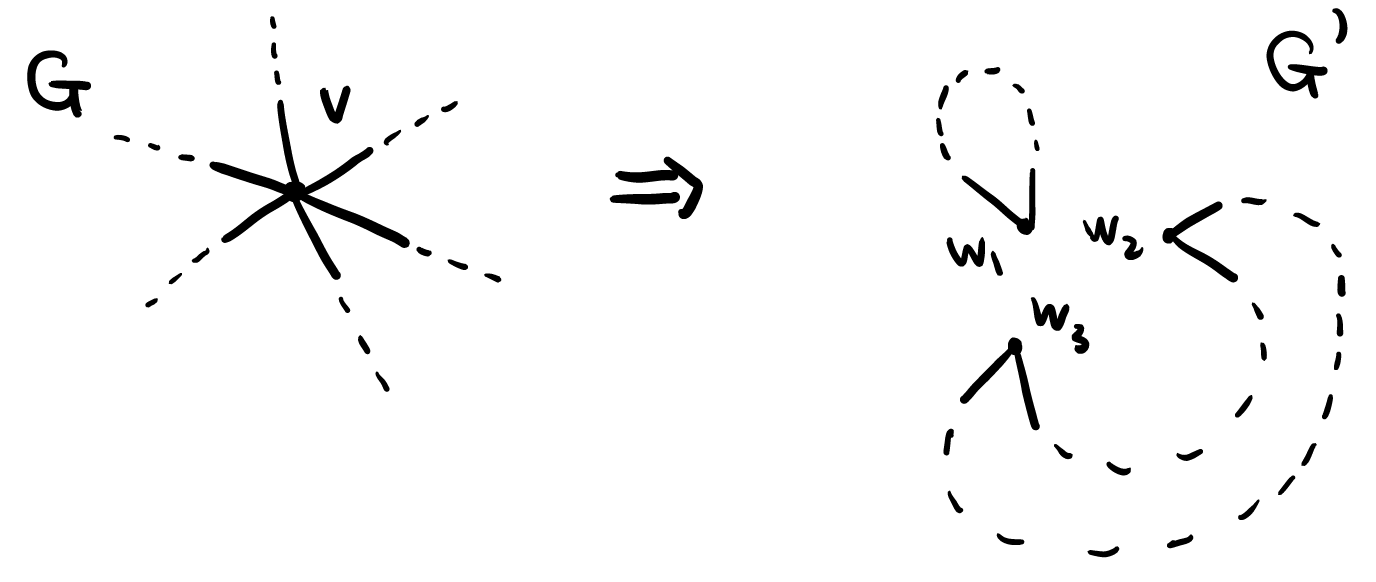
\includegraphics[height=4cm]{Figure1.png}\\
    \caption{Splitting $v$ into into vertices $w_1,..., w_n$, resulting in connected component(s).}
    \end{figure}

    Each component $G_i$ of $G'$ is nonempty because it contains at least one vertex, $w_j$, and the two edges adjacent to $w_j$. Each $G_i$ is also finite because each of its vertices is a vertex in G, and G is finite. Note that we obtained $G'$ from G by replacing $v$, which had valence $\geq 4$, with vertices $w_j$ that each have valence 2, so the resulting $G'$ has one fewer vertex with valence $\geq 4$ than G, so it has $k+1-1=k$ such vertices. Since each $G_i$ is a component of $G'$, it can have at most the same number of such vertices as $G'$. Thus, each $G_i$ has $\leq k$ vertices with valence $\geq 4$.


    By the inductive hypothesis, each connected component $G_i$ of $G'$ has an Eulerian circuit with $m_i$ vertices
    \[
    \alpha_i=v_{i_0}, v_{i_1},...,v_{i_{m_i}}.
    \]
    By a cyclic shift, let $v_{i_0}=v_{i_{m_i}}=w_j$. We can thus rewrite the Eulerian circuits as
    \[
    \alpha_{ij}=w_j, v_{i_1},...,v_{i_{m_i-1}},w_j.
    \]

    Now, we can merge the connected components of $G'$ back into the original graph G by setting each vertex $w_i$ equal to the original vertex $v$. We can thus rewrite the Eulerian circuits above as
    \[
    \alpha_{ij}'=v, v_{i_1},...,v_{i_{m_i-1}}, v,
    \]
    Each of which is a path in G that starts and ends at $v$. Now we will construct a new circuit $\alpha$ through G by combining each circuit $\alpha_i'$:
    \[
    \alpha=v, v_{1_1},...,v_{1_{m_1-1}}, v, v_{2_1},...,v_{2_{m_2-1}}, v,...,v, v_{n_1},...,v_{n_{m_i-1}}, v.
    \]
    Note that the only modification of G to form $G'$ was splitting the vertex $v$ into multiple vertices. Thus, $G'$ has the same edges as G, and every edge in G is in one of the connected components of $G'$. Since each circuit $\alpha_i$ in $G_i$ was Eulerian, each of them traversed each edge in the connected component $G_i$ exactly once. Thus, $\alpha$ traverses each edge in G exactly once. Therefore, $\alpha$ is an Eulerian circuit in G. 
    \end{proof}
    
	
	\begin{thebibliography}{99}
	 \bibitem{Taylor} Taylor, Scott A. \emph{The Structures of Mathematics}, available online at \url{http://web.colby.edu/sataylor}

	
	\end{thebibliography}
	
\end{document}



















